\documentclass{article}

\usepackage[a4paper, left=1.5cm, right=1.5cm, top=2cm, bottom=2cm]{geometry}

\usepackage{../../../components/components} % <-- ton fichier .sty, avec toutes tes définitions

\usepackage{fancyhdr}


% Configuration des en-têtes et pieds de page
\pagestyle{fancy}
\fancyhf{} % reset tout

\fancyhead[L]{DL2 Math-Info CP3}
\fancyhead[C]{Introduction à GIT}
\fancyhead[R]{2025-2026}

\fancyfoot[L]{Ewen Rodrigues de Oliveira}
\fancyfoot[R]{\thepage}

\begin{document}

\docTitle{Introduction à GIT}
\section{Généralités}
\definition{
    GIT est un logiciel qui permet de suivre les mises à jour d'un projet, il est stocké dans un dépôt local \textit{(.git)}.
}
\vocabulary{On appelle \textbf{repository} (ou \textit{repo} pour les intimes) un dépôt GIT.}

\theorem{Fonctionnement}{}{true}{
    Quand on modifie des fichiers dans VS Code \textit{(i.e. dans le Working Directory)}, GIT détecte les changements (on les voit dans git status).\\

    On peut alors choisir quels changements on veut enregistrer (staging area) avec la commande \texttt{git add <fichier>}.\\\\
    Quand on a fait le tour des fichiers à sauvegarder, on peut faire un \textbf{commit} avec la commande \texttt{git commit -m "message"}. (on envoie les fichiers du staging area vers le dépôt local)

    \begin{center}
        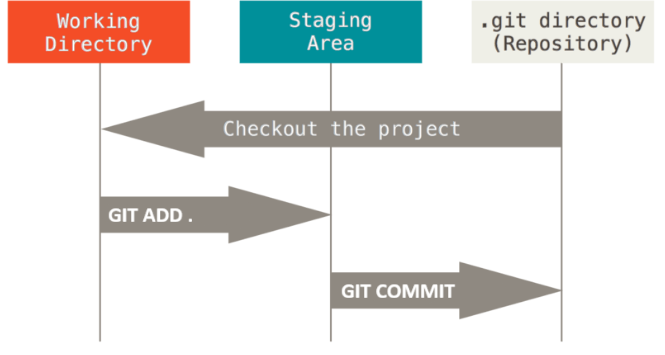
\includegraphics[width=0.5\textwidth]{./images/git.png}
        \captionof{figure}{Cycle de vie d'un fichier dans GIT}
    \end{center}
}

\remark{GIT stocke les changements, pas les fichiers entiers !}

\subsection{Mise en commun}

\definition{
    Pour partager son travail avec d'autres personnes, on utilise un dépôt distant (par exemple GitHub, GitLab, etc.).\\

    Intuitivement, on peut imaginer que le dépôt distant est une copie du dépôt local. Il stocke les mêmes différences, sauf qu'on peut les partager.
}

\theorem{Mise à jour du dépôt distant}{}{true}{
    Pour envoyer les changements du dépôt local vers le dépôt distant, on utilise la commande \texttt{git push}.\\

    Pour récupérer les changements faits par d'autres personnes sur le dépôt distant, on utilise la commande \texttt{git pull}.
}

\attention{
    Il faut toujours faire un \texttt{git pull} avant de faire un \texttt{git push}, sinon GIT va refuser d'envoyer les changements. (on doit avoir la dernière version du dépôt distant avant d'envoyer nos changements)
}

\subsection{Conflits et résolutions}

\definition{
    Après avoir fait un \texttt{git pull}, il se peut que GIT ne puisse pas fusionner les changements automatiquement. On parle alors de \textbf{conflit}.
}

\example{
    Si Jean modifie la ligne 3 d'un fichier et que Paul modifie aussi la ligne 3 du même fichier, GIT ne sait pas quelle version garder. Il y a donc un conflit.\\
    Le premier qui fait un \texttt{git pull} n'aura pas de problème, mais le deuxième aura un conflit à résoudre. (ici, Paul)
}

\remark{
    Pour éviter d'avoir des conflits, il faut toujours faire un \texttt{git pull} avant de commencer à travailler sur un projet. Pour être celui qui devra traiter le moins de conflit, il faut faire des \texttt{git push} régulièrement, avant les autres ;).
}

\theorem{Résolution de conflits}{}{true}{
    Quand un conflit survient, GIT modifie les fichiers concernés et demande à l'utilisateur de résoudre le conflit manuellement.\\

    Dans VS Code, les parties en conflit sont marquées avec des indicateurs \texttt{<<<<<<}, \texttt{======} et \texttt{>>>>>>}.\\

    Il faut choisir quelle version garder (ou fusionner les deux) et supprimer les indicateurs, puis faire un commit.\\

}

\example{
    
    \begin{center}
        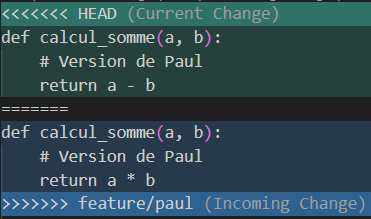
\includegraphics[width=0.5\textwidth]{./images/conflit.png}
        \captionof{figure}{Exemple de conflit dans VS Code}
    \end{center}
}



\remark{VS Code propose une interface graphique pour résoudre les conflits, ce qui peut être plus simple que de le faire manuellement.}

\section{Branches}

\definition{
    Une branche est un ensemble de commits. Par défaut, GIT crée une branche appelée \texttt{main} (ou \texttt{master} dans les anciennes versions).
}

\theorem{Utilisation des branches}{}{true}{
    Les branches permettent de travailler sur des fonctionnalités ou des corrections de bugs sans affecter la branche principale.\\

    On peut créer une nouvelle branche avec la commande \texttt{git branch <nom\_branche>}, puis se déplacer dessus avec \texttt{git checkout <nom\_branche>}.\\
}

\remark{Depuis GIT 2.23, on peut utiliser la commande \texttt{git switch <nom\_branche>} pour se déplacer sur une branche.}

\theorem{Fusion de branches}{}{true}{
    Une fois le travail sur une branche terminé, on peut fusionner les changements dans la branche principale avec la commande \texttt{git merge <nom\_branche> -m "message"}.\\

    Il est recommandé de faire un \texttt{git pull} avant de fusionner pour éviter les conflits.\\
    C'est comme un commit, mais pour une branche entière.
    \begin{center}
        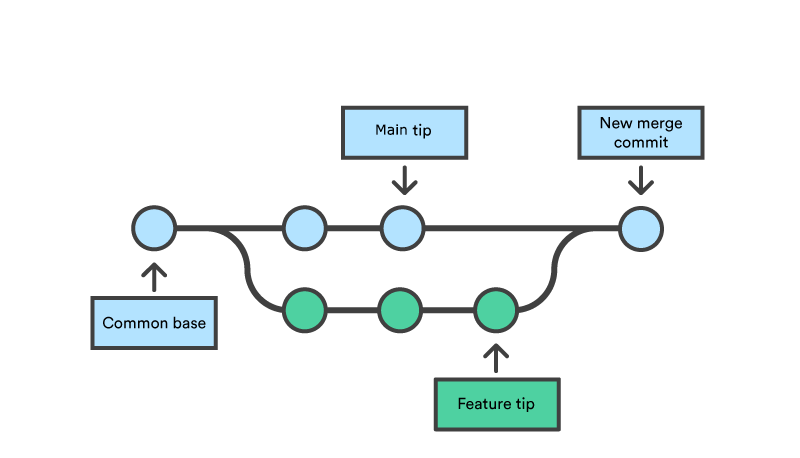
\includegraphics[width=0.5\textwidth]{./images/merge.png}
        \captionof{figure}{Fusion de branches}
    \end{center}
}


\end{document}
